\section{Numbers and units}
Numbers and units should be formatted following the NIST guide to the SI \cite{NIST_SI}.

Quantity values with units should not be split over lines. Use a non-breaking spacing to prevent this in MS Word (CTRL-SHIFT-SPACE). In \LaTeX, the symbol \verb|~| can be inserted to provide a non-breaking, however, the `siunitx' package provides better support for units (and number formatting).

When numbers are expressed with more than four digits (either side of the decimal marker), a thin space is preferred to a comma, or nothing, as separator between groups of three digits. Some examples are shown in table~\ref{tab:ex_number_formats} 
\begin{table}[ht]
\begin{center}
% default is group-minimum-digits=5
% so here we make sure that the 8 in 8012 
% is not aligned differently from other numbers
\begin{tabular}{S[group-minimum-digits=4]l}
{do this} &  {not this} \\ \hline 
76483522 & 76,483,522 \\
43279.168 & 43,279.168 \\
8012 & 8,012 \\ 
18012 & 18,012 \\
0.4917223 & 0.4917223 
\end{tabular}
\caption{Preferred number formatting. Note that all numbers in the left-hand column are vertically aligned to the location of the decimal point and that a thin space separates thousands. In this example, in the left-hand column, a thin-space separator has been used for all numbers, but an acceptable format for the third row is also \num{8012}.}
\label{tab:ex_number_formats}
\end{center}
\end{table}

The \LaTeX\ package `siunitx' defines a new column type `S' that applies numerical formatting rules to numbers in a tabular environment. The numbers in the left-hand column of table~\ref{tab:ex_number_formats} were produced in this way. The column heading `do this' was enclosed in brackets to indicate that it did not need numerical formatting (i.e., \verb|{do this}|). A thin space was also used when formatting the number \num[group-minimum-digits=4]{8012}.
\footnote{Default formatting will not introduce a thousands separator until there are more than 4 digits. This was changed by writing \texttt{S[group-minimum-digits=4]} in the column specifier.} 


\subsection{Generating a space separator}
It is not easy to generate a thin space in Microsoft Word.\footnote{There is no difficulty in \LaTeX: correct formatting of numbers and units is handled by the package `siunitx'.} The following recipe is one possibility:
\begin{enumerate}
\item Type a space normally (use a non-breaking space if needs be) 
\item Select the space and right click to obtain the context menu; select Font …
\item Select the Advanced tab and set Spacing to `Condensed' (the ``by 1 pt'' default is OK)
\item Click OK and copy the space to the clipboard 
\end{enumerate}

This thin space character can be pasted into numbers as required.

Using Microsoft Excel it is possible to select a normal-width space separator for groups of `thousands'  in the number formatting. Unfortunately, this does not insert spaces between groups of three digits to the right of the decimal marker. 

To set up Excel to insert a space between digits to the left of the decimal marker:
\begin{enumerate}
\item Find the `Use system separators' check box under `Editing Options' in the Excel Options menu 
\item Un-check this box and type a space character into the `Thousands Separator' box
\end{enumerate} 

Alternatively, to insert spaces between groups of three digits to the right of the decimal marker use a custom number format of ``\verb|#.### ### ###|''. Similarly, a custom number format of ``\verb|# ### ###|'' can be used to set a space as the thousands separator.

\section{Mathematical language}
Mathematical formulae and equations should be contained in complete English sentences with appropriate punctuation. 

Punctuation follows equations: a computation that ends a sentence needs to end with a full stop; otherwise an equation should be followed by a comma (an effective way to check for appropriate punctuation is to read text containing equations out loud). 

For example, the following sentence appears in a report for a transformer test set: 
\[
\text{For $\rho = \SI{-1}{\%}$ and $\varphi= \SI{1}{crad}$,\; }
\varepsilon = \frac{1-0.01}{\cos(0.01)} - 1 \; =\; \SI{-0.995}{\%}\,. 
\]

Often, the use of space and separate lines for equations can be helpful to a reader, as it is in this extract from a calibration report:
\begin{quote}

A comparator is used to evaluate the vector ratio $Q_\mathrm{X}/Q_\mathrm{N}$ where $Q_\mathrm{X}$ is the fundamental component of the signal vector at terminals X (either voltage or current) and $Q_\mathrm{N}$ is the fundamental component of the corresponding signal vector at terminals N. 

This ratio can be represented in polar co-ordinates as:
\[
\frac{Q_\mathrm{X}}{Q_\mathrm{N}} = (1 + \varepsilon) e^{\mathrm{j}\varphi} \;,
\]
where:

\begin{tabular}{rl}
$\varepsilon$ & is the ratio error, and \\
$\varphi$ & is the phase error, for the polar co-ordinate system. 
\end{tabular}

\vspace{\baselineskip}
This ratio can be also represented in rectangular co-ordinates as:
\[
\frac{Q_\mathrm{X}}{Q_\mathrm{N}} = 1 + \rho + \mathrm{j}\cdot\tan (\gamma) \;,
\]
where
\begin{tabular}{rl}
	$\rho$ &  is the ratio error, and \\
	$\tan (\gamma)$ & is the phase error, for the rectangular co-ordinate system. 
\end{tabular}

\vspace{\baselineskip}	
This ELTEL comparator reports the ratio error as $\rho$ (rectangular co-ordinate system) and the phase error as $\varphi$ (polar co-ordinate system).
\end{quote}

\subsection{Symbols and notation}
It is important to choose an appropriate set of symbols to represent quantities. That includes the alphabet, the font (Roman, bold, italic, etc) and the case. Getting the notion right can be hard: be prepared to spend more time on sorting this out than you might expect.

It pays to choose the style and a selection of symbols as early as possible when writing documents ( see~\S\ref{sss:style_guide} ). This may require careful consideration of what exactly will be described. Each symbol should only represent one thing, otherwise the intended meaning in your writing can become obscure and possibly ambiguous. 

Communicating efficiently with the reader is paramount: if there is an existing convention, follow it. Wherever possible, try to be consistent. If one document is closely related to another, then try to maintain consistent notation. 

\subsubsection{MSL style guide for symbols}
\label{sss:style_guide}
Here is a default guide for MSL publications. Follow this unless the rules are unsuitable for the work, or a distinct set of rules needs to be used (e.g., a scientific journal may ask for a specific style).

\begin{itemize}
\item Italicize symbols representing quantities or other variables (either Greek or Latin symbols). 

Abbreviated symbols, or full words, used as descriptors (often as subscripts or superscripts), should be in Roman font (not italics). For example, $V_\mathrm{input}$  (The `$V$' is italic, but not the subscript).

However, when variables, rather than descriptors or labels, appear in subscripts or superscripts they should be italicised. So, for example, the $i^\mathrm{th}$ instance of `$x$' could be written as $x_i$ (both `$x$' and `$i$' italicised).

\item Units and unit symbols should not be italicized, so $V_\mathrm{input}$ = \SI{12.1}{ V }.
	
\item Constants should be in Roman font. So, special symbols representing numbers, like $\mathrm{\pi}$, $\mathrm{e}$ and $\mathrm{i}$ or $\mathrm{j}$ (the imaginary unit), should be set in Roman font.
	
\item Operators should be set in Roman font. For instance, $\mathrm{d}y/\mathrm{d}x$ (the d's are in upright font).
	
\item Complex variables should use bold italic, such as $\bm{z}=\bm{x}+\mathrm{i} \bm{y}$. Some font families do not offer a bold italic font option, so this can be a problem.
	
\item Matrices and vectors should be written in bold Roman font.

\end{itemize}Note the equation editor in MS Word (or MathType, which is an extended commercial version) automatically applies some of these rules, but not all. 


\section{Scientific documents}
 \label{s:scientific_documents}
An excellent paper about the craft of writing scientific prose appeared in Scientific American in 1990 \cite{GopenAndSwan}. It develops seven structural principles that can be followed to make complicated scientific prose easier to read and understand. The principles are listed below as a convenient reminder, but the paper should be read to understand them properly.
\begin{enumerate}

\item	Follow a grammatical subject as soon as possible with its verb.
\item	Place in the stress position the ``new information'' you want the reader to emphasize (readers naturally emphasize material at the end of a sentence: this is the ``stress position'').
\item	Place the person or thing whose ``story'' a sentence is telling at the beginning of the sentence, in the topic position (information in the ``topic'' position usually begins a sentence and establishes a perspective for viewing the sentence as a unit). 
\item	Place appropriate ``old information'' (material already stated in the discourse) in the topic position for linkage backward and contextualization forward (when ``old'' information is continually placed in the topic position it helps the reader construct the logical flow of an argument). 
\item	Articulate the action of every clause or sentence in its verb. 
\item	In general, provide context for your reader before asking that reader to consider anything new. 
\item	In general, try to ensure that the relative emphases of the substance coincide with the relative expectations for emphasis raised by the structure.
\end{enumerate}

\subsection{Equations and prose in scientific documents}
David Mermin offered several simple principles about writing equations in scientific papers in his entertaining Reference Frame column in Physics Today \cite{Mermin}.
\begin{enumerate}

\item	Number all displayed equations (not just the ones you, the author, wish to refer to).
\item When referring to an equation, identify it by a phrase as well as a number (to help the reader remember what the equation was about).
\item	End a displayed equation with a punctuation mark (so the prose with equations embedded flows).

\end{enumerate}

\subsection{Tables}
As a general principle, use as little unnecessary decoration in tables as possible: it is the numbers or data that are of interest, not the graphic design. Tables should encourage the eye to compare data and help the reader to think about the information (rather than the design) being presented. 
Alignment is important when presenting numbers, because the eye picks up on vertical and horizontal patterns. If lines are drawn on a table, to frame or separate numbers, they can distract the reader from the data being presented. 
The following guidelines should be considered
\begin{itemize}
\item	Columns of decimal numbers should be aligned on the decimal point; columns of integers should be aligned on the right (the one's digit); text should usually be left-aligned.
\item	Draw as few horizontal and vertical lines as possible (consider using horizontal space instead of horizontal lines to separate blocks of information).
\item	Consider using captions to supplement column headings, by keeping column headings brief and putting extra details in the caption.
\item	The caption should be placed above the table. The caption text may use a smaller sized font than the many body and should be left-aligned.
\item	Units should be included in a column heading; unit symbols are preferred to full unit names, but be consistent.
\item	Use footnotes to convey information about specific entries in the table (e.g., entries that are out of scope).
\end{itemize}   
Table~\ref{tab:electrical_results} illustrates some of these guidelines. Note the vertical alignment of numbers and the caption above the table.\footnote{This table was produced in \LaTeX\ using the `siunitx' package. However, it is a copy of a table generated, with a very similar appearance, using MS Word. There is a tab-stop available in MS Word that aligns numbers on the decimal point.}

\clearpage
\begin{sidewaystable}[h!]
%\sisetup{group-minimum-digits=4}
\centering
\caption{Nominal voltage applied: \SI{110}{V}, \SI{50}{Hz}}
  \label{tab:electrical_results}
  \begin{tabular}{SSSSSSSS}
  	\toprule \\
  	{Indicated voltage} & {Indicated phase} & {Voltage ratio error} & {Expanded} & {Coverage} & {Phase error} & {Expanded} & {Coverage} \\
  	{ratio error} & {error} & {correction} & {uncertainty} & {factor} & {correction} & {uncertainty} & {factor} \\
  	{$(\rho / \si{\%})$} &  {$(\varphi / \si{crad})$} &  {$(\rho / \si{\%})$} &  {$(U(\rho)/\si{\%})$}
  	&  {$(k)$}  &  {$(\varphi / \si{crad})$} &  {$(U(\varphi)/ \si{crad})$} &   {$(k)$} \\
	\\
    \midrule
    -10.00 & -10.00 & 0.028 & 0.021 & 2.0 & -0.085 & 0.020 & 2.0 \\
    -10.00 & 0.0000 & 0.000 & 0.021 & 2.0 & -0.074 & 0.020 & 2.0 \\
    -10.00 & 10.00 & -0.032 & 0.021 & 2.0 & -0.060 & 0.020 & 2.0 \\
    0.0000 & -10.00 & 0.0286 & 0.0017 & 2.6 & -0.046 & 0.007 & 2.1 \\
    0.0000 & 10.00 & -0.0367 & 0.0040 & 3.0 & -0.020 & 0.006 & 2.1 \\
    10.00 & -10.00 & 0.030 & 0.021 & 2.0 & -0.018 & 0.020 & 2.0 \\
    10.00 & 0.0000 & -0.007 & 0.021 & 2.0 & -0.0007 & 0.020 & 2.0 \\
    10.00 & 10.00 & -0.042 & 0.021 & 2.0 & 0.010 & 0.020 & 2.0 \\
    \bottomrule
  \end{tabular}
\end{sidewaystable}
%\begin{sidewaysfigure}[h]
%\centering
%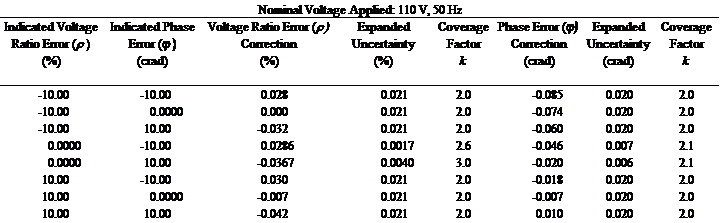
\includegraphics[width=.7\textwidth]{pictures/table_electrical_results}
%\label{tab:electrical_results}
%\caption{An example of tabulated measurement results. Note the vertical alignment of numbers and the caption above the table.}
%\end{sidewaysfigure}
\clearpage

\subsection{Figures}
Graphs can help a reader to understand the structure of data. It is relatively rare to include graphs in calibration reports but, in scientific papers and reports, graphs are a powerful tool for communication.

Cleveland has written an excellent book about graphing data \cite{Cleveland}. He offers a set of guiding principles on designing graphs, which are summarised here (but consult the book – it is worth the effort). Note that Cleveland was more concerned with the sort of graphing used in scientific papers and reports. However, many of these principles also apply to graphs in calibration reports.

Graphs can help a reader to understand the structure of data. It is relatively rare to include graphs in calibration reports but, in scientific papers and reports, graphs are a powerful tool for communication.


\begin{enumerate}

\item	\textit{Make the data stand out and avoid superfluity}

For instance, don’t allow elements in the graph to interfere with the data; make sure the elements encoding data are visually prominent; don’t allow a graph to be cluttered by unnecessary bits and pieces.

\item	\textit{Use visually prominent elements to show the data}

Be careful that symbols used to encode data are visually distinct; that they do not obscure each other; that lines used to join data points do not detract from the prominence of the data points.

\item	\textit{Use a pair of lines in the scale-line rectangle for each variable. Make the data rectangle slightly smaller than the scale-line rectangle. Tick marks should point outward.}

Data should not interfere with the scale markings. So, allow a little space between the surface used to display the data and the bounding rectangle with the scale markings. For the same reason, place tick marks outside the rectangle, as shown in figure~\ref{fig:cleveland_promience} below ( Fig 2.8 in \cite{Cleveland} ).

\begin{figure}[ht]
\centering
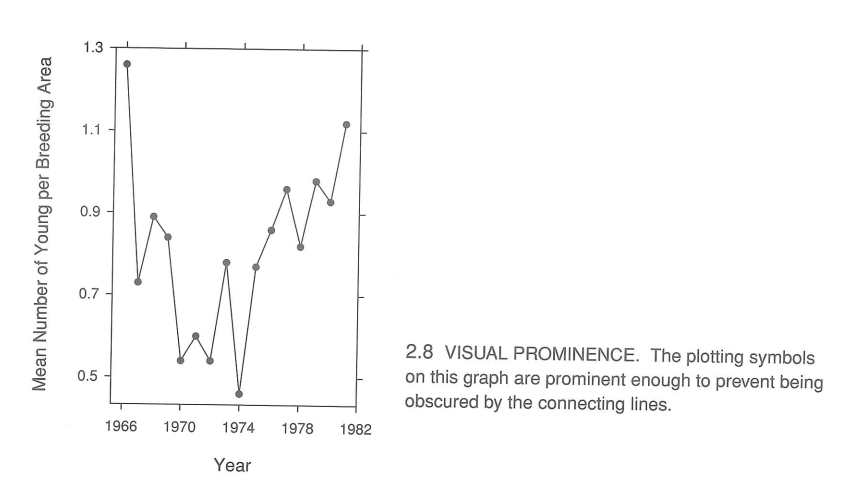
\includegraphics[scale=1]{pictures/visual_prominence}
\caption{From Cleveland \cite{Cleveland}. Note the clear visual separation of the data from the scale and other markings.}
\label{fig:cleveland_promience}
\end{figure}

\item	\textit{Do not clutter the interior of the line-scale rectangle}

Avoid the temptation to include too much on a graph: a legend, reference lines, arrows and labels, can contribute to a figure that is hard to visually disentangle.

\item	\textit{Do not use too many tick marks}

Tick marks convey a sense of the measurement scale; you don’t need many (3 to 10, perhaps).

\item	\textit{Use a reference line when there is an important value that must be seen across the entire graph, but do not let the line interfere with the data.}

\item	\textit{Do not allow data labels inside the graph to interfere with the data or to clutter the graph}

\item	\textit{Avoid notes and keys inside the graph. Put a key outside and put notes in the caption.}

\item	\textit{Overlapping plotting symbols must be visually distinguishable} 

\item	\textit{Superimposed data sets must be readily visually assembled}

When there are several sets of data displayed, make sure that elements used to plot data points are visually distinct.

\item	\textit{Visual clarity must be preserved under reduction and reproduction}

This point was more of an issue before modern scanning technologies, but it is not uncommon to sample an image and then insert a (scaled) copy of that image in another document (e.g., our use of Cleveland's Fig 2.8 above).

\end{enumerate}

\subsubsection{Captions}
Figure captions should be placed below the corresponding figure and may use a smaller sized font than the many body text. Units should be included in the axis labels; it is not necessary to repeat that information in the caption.

Figure captions should be comprehensive and informative. The reader should not have to scour the document for information required to understand the displayed. Nevertheless, a series of related captions need not repeat information unnecessarily. If the first caption provides a comprehensive description, following captions may simply refer to it.

Cleveland recommends the following framework for figure captions \cite{Cleveland}:
\begin{itemize}
\item	\textit{Describe everything that is graphed}
\item	\textit{Draw attention to the important features of the data}
\item	\textit{Describe the conclusions that are drawn from the data on the graph}

This recommendation is made in the context of research work. MSL calibration reports are more likely to contain graphs that provide access to quantitative information, rather than present conclusions visually. Guidance in that case might be expressed as something like this:
\begin{quote}
\textit{Describe how the graph can be interpreted and used by the reader}
\end{quote}

\end{itemize}

\subsection{Uncertainty}
Clear statements about measurement uncertainty and related concepts are sadly lacking in the metrology literature. This is a problem, because readers are presented with jargon that is rarely helpful to them. Often too, it seems that poor style is self-perpetuating. Presumably because authors do not have clear stylistic guidelines available and are unclear in their own minds about the subject. 

MSL should adopt a clear style when writing about uncertainty. These notes help avoid common problems.

\paragraph{Which uncertainty?}
Often, the intended meaning of `uncertainty' is not clear. Statements like ``all measurements have uncertainties'' may be used without a reasonable definition in the surrounding context.

There are two specific types of uncertainty: standard uncertainty and expanded uncertainty. It is better to write the full term, which, as a side-effect, will also discourage any tendency to be glib (``all measurements have standard uncertainties'' just doesn't have the same ring to it). 

\paragraph{What is uncertain?}
A measurement result (measured value) is never uncertain: this is a known number, call it $y$, which may be read from an instrument or calculated from data. Uncertainty only occurs when $y$ is used in place of the measurand (call that $Y$). The uncertainty is then about what happens when the value $y$ is used instead of $Y$. 

To write clearly and use the word uncertainty correctly, a useful trick is to replace `the uncertainty of $y$' in a sentence with `the uncertainty of $y$ as an estimate of $Y$'. (If overdone, this may become rather laborious, but, this form should be used unless the reader will understand the writer's intention from clear statements made close by in the text.) 

\paragraph{Prefer the word `error'} 
Measurement error is the difference between the measurand $Y$ and the measured value $y$. All measurements are subject to measurement error (we never expect that $y=Y$). So, while it is unhelpful to say something like ``all measurements have uncertainties'', what we could say is that ``all measurements are subject to measurement error''.

\paragraph{Measured values are estimates; values of uncertainty are calculated}

One often reads that uncertainty has been estimated. This is used in many authoritative works, but it is unhelpful and should be avoided. The term ``estimate'' should be reserved for a measurement result (as an estimate of the measurand). 

Measurement is a process that produces an estimate of a measurand. This is fundamental. When we talk about the uncertainty in a result, as an estimate of the measurand, we generally intend that the uncertainty is calculated according to a common set of rules (GUM). 

The verbs `measure' and `estimate' are synonymous from our perspective. Although, `measure' is preferred to `estimate', this does not justify the use of `estimate' to describe calculations of uncertainty.  

So, for instance, don't write
\begin{quote}
``This uncertainty was estimated by …'',
\end{quote}
instead write
\begin{quote}
``This expanded uncertainty was calculated by …''.
\end{quote}
There is a reason for writing  `estimating uncertainty' in authoritative works, but it is rather specialised and unhelpful to most metrologists (which is why we discourage this usage). The GUM associates a Gaussian distribution with the error generated by a measurement procedure. The standard deviation of this  distribution is not known. However, the standard uncertainty associated with a result can be considered an estimate of the actual standard deviation. This is analogous to the distinction made in statistics between a sample standard deviation and a population standard deviation. Note, however, that the GUM method for calculating expanded uncertainty deals with this inherent imprecision (by using statistical tables of Student-$t$). So, there is no need to bring it to the reader's attention by using the word `estimate'.

Another reason for discouraging expressions like `estimating uncertainty' is that it implies there is some actual `true' value of `uncertainty', which is misleading. Granted, one might, in the GUM context, claim to estimate the standard uncertainty of the Gaussian distribution of measurement error–--a statistical parameter that is presumed to exist. However, it is often the expanded uncertainty that is referred to as being `estimated' and an expanded uncertainty need not be associated with any unique physical parameter.

\paragraph{Level of Confidence}
The level of confidence associated with a statement of expanded uncertainty is often said to be estimated. This too should be avoided. For instance,
\begin{quote}
``The expanded uncertainties were calculated using a coverage factor $k = 2.1$ and define an interval estimated to have a \SI{95}{\%} level of confidence''
\end{quote}
would be better expressed as
\begin{quote}
``The expanded uncertainties were calculated using a coverage factor $k = 2.1$, for a \SI{95}{\%} level of confidence''.
\end{quote}
The use of `estimated' above may reflect the author's reticence to claim a level of confidence of precisely \SI{95}{\%}. If that is so, then a suitable phrase might be ``for a level of confidence of at least \SI{95}{\%}''. 

Note that the author's reticence is of no value to the reader of a report. The essential information is that the GUM process has been followed using a coverage factor $k$ of definite value. The reader may wish to calculate the standard uncertainty, so the report must provide enough information to do this: in this case by dividing the value of expanded uncertainty by the reported value of $k$.

\paragraph{Coverage factor and degrees of freedom}
The reader will need to know the number of degrees of freedom associated with the standard uncertainty of a measurement if they intend to carry out uncertainty calculations of their own. 

Sometimes a value of coverage factor is described as being `derived from the Student-$t$ distribution'. This is not very helpful. Consider instead reporting both the coverage factor and the number of degrees of freedom associated with the standard uncertainty of the measurement.

It is certainly true that statistical tables for the Student-$t$ distribution can be consulted, or a computer programme used, to obtain the number of degrees of freedom corresponding to a coverage factor. However, the author has this information already and can provide it directly; there is no need to mysteriously refer to a \textit{`derivation from the Student-$t$ distribution'} and expect the reader to reverse-engineer the calculation. 

\paragraph{The colloquial meaning of uncertainty}
A thing that is uncertain is not accurately known. So, a measurand may correctly be described to be uncertain. 

However, things that are unpredictable may also be described as uncertain, such as the weather. A measurand is not uncertain in this sense, because it is considered fixed. This is an important point and the source of confusion: never suggest that the measurand is variable or, worse, random. 

The unpredictability of a measurement result is associated with the inevitability of measurement error (the difference between the measured value and the measurand). So, measurement error may be correctly described as uncertain, in that it is both unknown and random.

There are two specific technical terms: expanded uncertainty and standard uncertainty. One is associated with uncertainty about a measurand and the other with an unpredictable measurement error. An expanded uncertainty is the half-width of an interval that is likely to cover the actual measurand. A standard uncertainty, on the other hand, is an estimate of the standard deviation of the Gaussian distribution of measurement error.

It is important not to confuse these two concepts.

\paragraph{The purpose of measurement}
Measurements are always performed for a reason: they inform decisions by providing information about the physical world. 

The correctness of any decision based on measurement results will be uncertain, because the corresponding measurands cannot be known exactly. This is where uncertainty about a measurand affects human activity; it is where the colloquial meaning of uncertainty applies to measurement. 

For instance, a decision must be be made between two possible actions: A or B. The decision will be based on the level of some quantity $X$, which is measured. Four possible outcomes depend on how the measured value $x$ compares with some fixed value $Y$: 
\begin{enumerate}[label=\roman*)]
\item A is correctly chosen, 
\item A is incorrectly chosen, 
\item B is correctly chosen, and 
\item B is incorrectly chosen.
\end{enumerate} 
Incorrect decisions can arise because of measurement error. Any decision process should be designed to minimise the occurrence of bad decisions, but they may occur nevertheless. 

When writing for a general audience, it is important to consider the link between the world of measurements and the world that we live in. This is surely the fundamental reason for paying any attention to uncertainty, yet it is rarely acknowledged. 

\subsection{The Abstract}
Figure~\ref{fig:abstract} is a very clear illustration of how to structure an abstract. The journal in this case may have accepted rather long abstracts but the guiding principles remain valid.

\begin{figure}[ht]
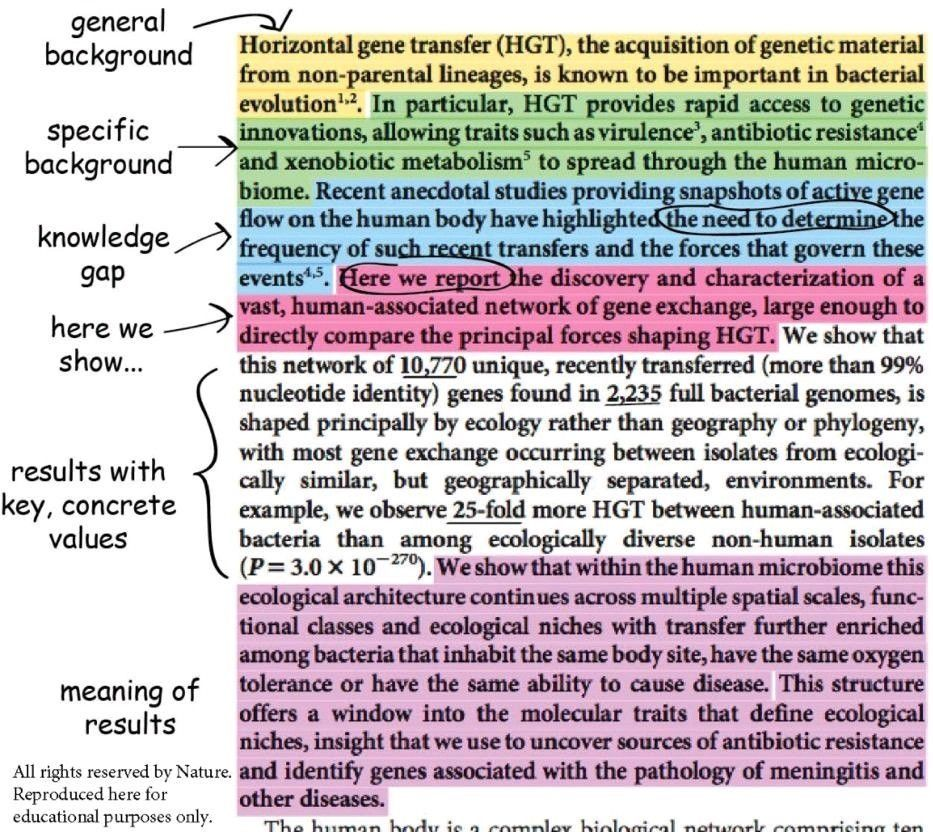
\includegraphics[scale=.4]{pictures/the_perfect_abstract.jpg}
\label{fig:abstract}
\caption{(Source is unknown)}
\end{figure}
